\documentclass{article}

% Packages for formatting
\usepackage{tcolorbox}
\usepackage{xcolor}
\usepackage{hyperref}
\usepackage{amsmath}
\usepackage{geometry}
\usepackage{tocloft}
\usepackage{colortbl}
\usepackage{graphicx}
\usepackage{lipsum} % For dummy text
\usepackage{tikz}
\usetikzlibrary{positioning}
\usetikzlibrary{shapes.geometric, arrows}

% Change hyperref settings to remove boxes
\hypersetup{
    colorlinks=true,
    linkcolor=black,
    filecolor=black,
    urlcolor=black,
    citecolor=black,
}

% Page layout
\geometry{a4paper, margin=1in}

% Colors
\definecolor{codehighlight}{rgb}{0.36, 0.54, 0.66}
\definecolor{coderule}{rgb}{0.7, 0.7, 0.7}           % Grey frame codebox
\definecolor{codebg}{rgb}{1.0, 1.0, 1.0}             % Background codebox
\definecolor{tableheader}{RGB}{128, 128, 128}        % Grey table header
\definecolor{tablecell}{RGB}{250, 250, 250}          % Table cell
\definecolor{title}{rgb}{0.36, 0.54, 0.66}           % Custom title color


% Code box style
\tcbset{
    colframe=tableheader, % Frame color
    colback=tablecell,    % Background color
    arc=0pt,           % Corner radius
    boxrule=1pt        % Frame thickness
}

% Table of contents
% \renewcommand{\cftbot}{}

% Main document
\begin{document}

% Cover pages
% Cover page
\begin{titlepage}
    \centering
    \vspace{\fill}  % push everything to top

    \thispagestyle{empty} % Remove page numbering

    % Background image
    \newgeometry{left=0cm, right=0cm, top=0cm, bottom=0cm} % Temporarily set margins to 0
    \includegraphics[width=\paperwidth,height=\paperheight]{images/cover.jpg}
    \restoregeometry % Restore the margins

    \vspace{\fill}   % push everything to bottom
\end{titlepage}
\newpage
\ % The empty page
\thispagestyle{empty} % Remove page numbering
\newpage
% Title page
\begin{titlepage}
    \thispagestyle{empty} % Remove page numbering
    \centering
    \vspace*{\fill}     % push everything to top

    \begin{center}
        \vspace*{2cm}   % Additional vertical space if needed
        {\Huge \textbf{My Notebook Template}}\\
        \vspace{1cm}
        {\Large Anchit Mulye}\\
        \vspace{0.5cm}
        {\Large \today}
    \end{center}

    \vspace*{\fill}     % push everything to bottom
\end{titlepage}
\newpage
\ % The empty page
\thispagestyle{empty} % Remove page numbering
\newpage
\pagenumbering{roman}
% Table of contents
\newpage
\thispagestyle{empty} % Remove page numbering
\title{My Notebook Template}
\author{Anchit Mulye}
\date{\today}
\maketitle

\tableofcontents
\newpage

% Chapters
\pagenumbering{arabic}
\section{Mathematical Questions}

\subsection{Solve the quadratic equation \(ax^2 + bx + c = 0\).}
\[
x = \frac{-b \pm \sqrt{b^2 - 4ac}}{2a}
\]

\subsection{Evaluate the integral \(\int e^x \, dx\).}
\[
\int e^x \, dx = e^x + C
\]

\subsection{Find the derivative of \(f(x) = \sin(x)\).}
\[
\frac{d}{dx} \sin(x) = \cos(x)
\]

\subsection{Solve the system of linear equations:}
\[
\begin{cases}
2x + 3y = 6 \\
4x - y = 5
\end{cases}
\]
\[
x = 2, \quad y = 0
\]

\subsection{What is the limit of \(\frac{\sin(x)}{x}\) as \(x\) approaches 0?}
\[
\lim_{x \to 0} \frac{\sin(x)}{x} = 1
\]

\subsection{Expand the binomial \((a + b)^3\).}
\[
(a + b)^3 = a^3 + 3a^2b + 3ab^2 + b^3
\]

\subsection{What is the sum of the first \(n\) terms of an arithmetic series with first term \(a\) and common difference \(d\)?}
\[
S_n = \frac{n}{2} [2a + (n-1)d]
\]

\subsection{Solve for \(x\) in the equation \(e^x = 5\).}
\[
x = \ln(5)
\]

\section{Diagrams}

\subsection{Simple Flowchart}

\tikzstyle{startstop} = [rectangle, rounded corners, minimum width=3cm, minimum height=1cm,text centered, draw=black, fill=red!30]
\tikzstyle{process} = [rectangle, minimum width=3cm, minimum height=1cm, text centered, draw=black, fill=orange!30]
\tikzstyle{decision} = [diamond, minimum width=3cm, minimum height=1cm, text centered, draw=black, fill=green!30]
\tikzstyle{arrow} = [thick,->,>=stealth]
\begin{center}
\begin{tikzpicture}[node distance=2cm]
    \node (start) [startstop] {Start};
    \node (process1) [process, below of=start] {Process 1};
    \node (decision1) [decision, below of=process1, yshift=-1cm] {Decision 1};
    \node (process2a) [process, below of=decision1, yshift=-1cm] {Process 2a};
    \node (process2b) [process, right of=decision1, xshift=3cm] {Process 2b};
    \node (stop) [startstop, below of=process2a] {Stop};

    \draw [arrow] (start) -- (process1);
    \draw [arrow] (process1) -- (decision1);
    \draw [arrow] (decision1) -- node[anchor=east] {Yes} (process2a);
    \draw [arrow] (decision1) -- node[anchor=south] {No} (process2b);
    \draw [arrow] (process2a) -- (stop);
    \draw [arrow] (process2b.east) -- ++(1,0) |- (process1.east);
\end{tikzpicture}
\end{center}


\subsection{Decision Tree}
\begin{center}
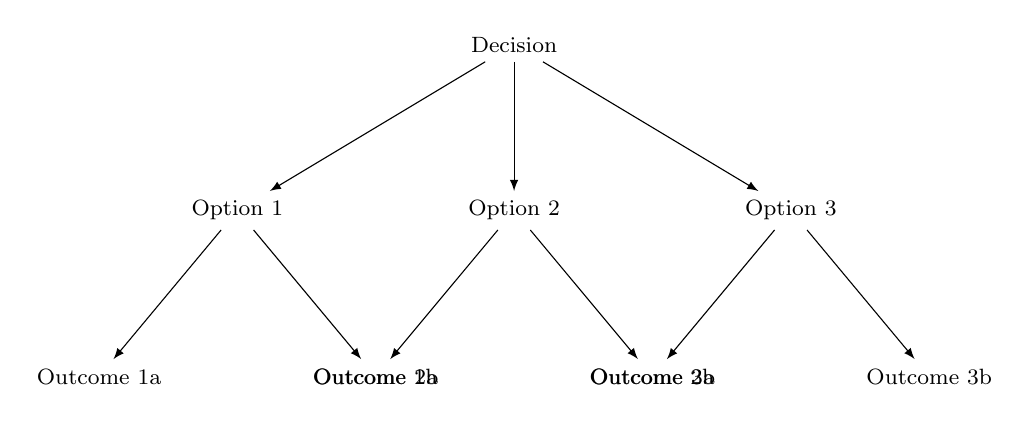
\begin{tikzpicture}[
    edge from parent/.style={draw, -latex},
    sibling distance=10em, level distance=6em,
    every node/.style={font=\footnotesize}]
    
    \node {Decision}
        child { node {Option 1}
            child { node {Outcome 1a} }
            child { node {Outcome 1b} }
        }
        child { node {Option 2}
            child { node {Outcome 2a} }
            child { node {Outcome 2b} }
        }
        child { node {Option 3}
            child { node {Outcome 3a} }
            child { node {Outcome 3b} }
        };
\end{tikzpicture}
\end{center}

\subsection{Data Flow Diagram}
\tikzstyle{process} = [rectangle, minimum width=3cm, minimum height=1cm, text centered, draw=black, fill=orange!30]
\tikzstyle{data} = [trapezium, trapezium left angle=70, trapezium right angle=110, minimum width=2cm, minimum height=1cm, text centered, draw=black, fill=yellow!30]
\tikzstyle{arrow} = [thick,->,>=stealth]

\begin{tikzpicture}[node distance=1.5cm]
    \node (input) [data] {Input Data};
    \node (process1) [process, right of=input, xshift=3cm] {Process 1};
    \node (data) [data, below of=process1, yshift=-1cm] {Stored Data};
    \node (process2) [process, right of=process1, xshift=3cm] {Process 2};
    \node (output) [data, right of=process2, xshift=3cm] {Output Data};

    \draw [arrow] (input) -- (process1);
    \draw [arrow] (process1) -- (data);
    \draw [arrow] (data) -- (process2);
    \draw [arrow] (process2) -- (output);
    \draw [arrow] (data.north) -- ++(0,1) -| (process2.south);
\end{tikzpicture}


\subsection{Class Diagram}
\begin{center}
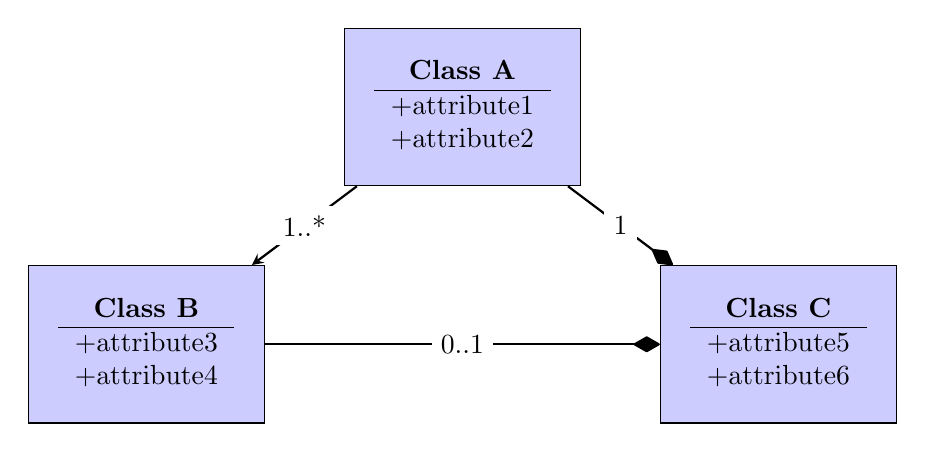
\begin{tikzpicture}[
    class/.style={
        rectangle,
        draw=black,
        fill=blue!20,
        text centered,
        minimum width=3cm,
        minimum height=2cm
    },
    relation/.style={
        -{stealth[open]},
        thick
    },
    aggregation/.style={
        -{diamond[open]},
        thick
    },
    composition/.style={
        -{diamond[fill=black]},
        thick
    },
    generalization/.style={
        -{stealth[open]},
        thick
    }
]

\node[class] (classA) {
    \begin{tabular}{c}
    \textbf{Class A} \\
    \hline
    +attribute1 \\
    +attribute2
    \end{tabular}
};
\node[class] (classB) [below left=of classA] {
    \begin{tabular}{c}
    \textbf{Class B} \\
    \hline
    +attribute3 \\
    +attribute4
    \end{tabular}
};
\node[class] (classC) [below right=of classA] {
    \begin{tabular}{c}
    \textbf{Class C} \\
    \hline
    +attribute5 \\
    +attribute6
    \end{tabular}
};

\draw[relation] (classA) -- (classB) node[midway, fill=white] {1..*};
\draw[aggregation] (classA) -- (classC) node[midway, fill=white] {1};
\draw[composition] (classB) -- (classC) node[midway, fill=white] {0..1};

\end{tikzpicture}
\end{center}
\include{questions/section3}

\end{document}